% ПЛАН
%# Глава 4 – Применение алгоритмов оценки параметров многотональных сигналов для анализа гармоник и интергармоник в электрических сетях на железнодорожном транспорте
%
%Выводы по главе:
%
%- В современных стандартах по анализу спектра в электрических сетях большее внимание уделяется нахождению интергармонических составляющих. Поскольку интергармонические составляющие имеют малую энергию по отношению к другим гармоникам и шуму, к алгоритмам для нахождения параметров гармоник возрастают требования по точности определения амплитуды в условиях высокого шума.
%- В стандартах также указывается требования о нахождение всех гармоник по 40 включительно, что, вместе с требованием о нахождении интеграмоник приводит к большому числу анализируемых гармонических составляющих сигнала.
%- Исходя из требований стандарта и анализа свойств изученных алгоритмов для анализа спектра сигнала в силовых электрических сетях железнодорожного транспорта рекомендуется использование метода дополнения сигнала нулями с применением разряженного преобразования Фурье.
%- Время расчета спектра реального сигнала этим методом на современном компьютере начального уровня составляет единицы секунд, что позволяет говорить о его приемлемом быстродействии для решения практических задач.

\chapter{Применение алгоритмов оценки параметров многотональных сигналов для анализа гармоник и интергармоник в электрических сетях на железнодорожном транспорте}\label{ch:ch4}

В четвертом разделе рассматривается понятие, характеризующее качества электрической энергии в электрических сетях систем электроснабжения переменного тока с частотами 50 и 60~Гц и порядок оценки результатов. Стандарты в области контроля определяющие состав показателей качества электрической энергии, методику измерений и характеристики средств измерений. В результате анализа производится сравнение государственных стандартов Российской Федерации (ГОСТ~Р) и международных стандартов (МЭК, IEC -- International Electrotechnical Commission), которые описывают требования и нормы КЭ \cite{IEC}.
%\hyperlink{https://www.iec.ch/}{[199]}. 
% [199 - International Electrotechnical Commission [Электронный ресурс] – Режим доступа:https://www.iec.ch/]

В четвертом разделе произведен сравнительный анализ существующих средств контроля учета показателей КЭ. В заключении описывается основные задачи и виды контроля КЭ.

Основным направлением в применении цифровой обработки сигналов является спектральный анализ. Каждый сигнал, который изменяется во времени, имеет частотный спектр. Электрические сигналы можно анализировать в частотной области с помощью анализаторов спектра, во временной области с помощью осциллографов. К анализатору спектра предъявляют различные требования измерений по максимальной  частоте входного сигнала. Ряд Фурье, представляет разложение несинусоидальной периодической функции на синусоидальные компоненты и позволяет рассматривать сигналы из временной области в частотной. Термин <<частотная область>> используется не только как <<область значений частот>> в преобразовании Фурье, но и как <<область значений переменных>>.

В последние годы правительством Российской Федерации разрабатывались и принимались нормативные правовые документы, которые
определяют государственную важность обеспечения высокой
энергетической, экономической и экологической эффективности производства,
передачи, распределения и потребления электрической энергии. Основопологащие документы:
\begin{itemize}
	\item Энергетическая стратегия политики России определяет цели и задачи развития страны в период до 2030 года, утвержденная распоряжением Правительства Российской Федерации от 13 ноября 2009~г. N 1715-р \cite{energy_strategy}. 
	\item Федеральный закон от 26 июля 2019~г. №~261-ФЗ «Об энергосбережении и о повышении энергетической эффективности и о внесении изменений в отдельные законодательные акты Российской Федерации (с изменениями на 26 июля 2019~года)»\cite{energy_saving_law_2019}.
\end{itemize}


Темпы потребления электроэнергии зависят от географического расположения региона. Главным направлением перспективного развития энергетики в России является, повышение эффективности контроля качества электрической энергии (КЭ). 
Министерство энергетики Российской Федерации (Минэнерго России) является федеральным органом исполнительной власти по государственной политике и нормативно-правовому регулированию в области энергосбережения. Минэнерго России управляет государственным имуществом в сфере производства, а также использования топливно-энергетических ресурсов. Энергетическая политика России позволяет использовать природные энергетические ресурсы в соответствии с приоритетами развития страны для устойчивого роста экономики. 

Реализация настоящей стратегии, является повышение эффективности 
контроля качества электрической энергии (КЭ). Поэтому необходимо уделять большее внимание методам контроля и анализа показателей КЭ. 
Каждое электрооборудование предназначено для работы при определенных параметрах электрической энергии: номинальной частоте, напряжении, токе и других параметрах. Поэтому для нормальной работы необходимо обеспечить требуемое качество электрической (КЭ).  КЭ определяется совокупностью ее характеристик, при которых электрооборудование нормально функционирует. Несоответствие показателей КЭ или свойства электрической энергии, которые ухудшают КЭ и приводят к преждевременному износу электрооборудования. 

Существенный вклад в решение рассматриваемых проблем внесли отечественные ученые: В.Г.~Аввакумов, В.Д.~Бардушко, Г.Я.~Вагин, В.Э.~Воротницкий, Н.И.~Воропай, В.Н.~Горюнов, А.З.~Гамм, И.В.~Жежеленко, Ю.С.~Железко, В.Г.~Курбатский, В.З.~Манусов, И.С.~Рокотян, М.О.~Доливо-Добровольский, В.Т.~Черемисин, М.Г.~Шалимов, А.К.~Шидловский и другие. 

%% УЧЕНЫЕ:
%В.Г. Аввакумов (Аввакумов В. Г. Влияние несимметрии и несинусоидальности напряжения на работу силовых конденсаторов [Текст]: (Энергет. параметры конденсаторных установок систем энергоснабжения электр. ж. д.): Автореферат дис. на соискание учен. степени кандидата техн. наук / Омский ин-т инженеров ж.-д. транспорта.)
%В.Д. Бардушко (Бардушко, Валерий Данилович – доктор технических наук. Анализ и параметрический синтез систем тягового электроснабжения: диссертация ... доктора технических наук: 05.13.01. - Иркутск, 2001. - 264 с.) 
%Г.Я. Вагин (Вагин Геннадий Яковлевич (род. 10 марта 1938 г.) – доктор технических наук, профессор кафедры электроэнергетики и электроснабжения Нижегородского государственного технического университета. Заслуженный деятель науки РФ. Более 200 научных работ, в том числе 16 монографий и 16 учебных пособий.) 
%В.Э. Воротницкий (Воротницкий, Валерий Эдуардович – доктор технических наук. Методы и средства совершенствования управления распределительными электрическими сетями и повышения их экономичности: автореферат дис. ... доктора технических наук: 05.14.02 / НИИ электроэнергетики АО ВНИИЭ. - Москва, 1996. - 54 с.)
%Н.И. Воропай (Воропай, Николай Иванович – (род. 1 ноября 1943 года) – физик, член-корреспондент РАН, заслуженный деятель науки Российской Федерации, лауреат премии имени Г. М. Кржижановского, доктор технических наук)
%В.Н. Горюнов (Горюнов, Владимир Николаевич – доктор технических наук. Беспазовые электрические машины с многополюсными и униполярными индукторами на высококоэрцетивных магнитах: Теория, мат. моделирование, совершенствование конструкций: диссертация ... доктора технических наук: 05.09.01. - Омск, 1993. - 417 с.) 
%А.З. Гамм (Гамм, Александр Зельманович (9 октября 1938 года, Волгоград) – физик, лауреат премии имени Г. М. Кржижановского. Методы анализа режимов электроэнергетических систем по данным измерений: диссертация ... доктора технических наук : 05.14.02. - Иркутск, 1981. - 337 с.)
%И.В. Жежеленко (Игорь Владимирович Жежеленко (род. 1930) – украинский учёный в области электроснабжения промышленных предприятий, доктор технических наук, профессор, заведующий кафедрой «Электроснабжение промышленных предприятий» ПГТУ, ректор Ждановского металлургического института / Приазовского Государственного Технического университета (1981—2003).)
%Ю.С. Железко (Железко, Юрий Станиславович. Научно-методические основы стратегии снижения потерь и повышения качества электроэнергии в электрических сетях: автореферат дис. ... доктора технических наук: 05.14.02. - Москва, 1996. - 46 c.) 
%В.Г. Курбатский (Курбацкий, Виктор Григорьевич. Мониторинг качества электроэнергии в электрических сетях России для выбора мероприятий по обеспечению электромагнитной совместимости: автореферат дис. ... доктора технических наук: 05.14.02 / Сиб. отд-ние. Сиб. энергетический ин-т им. Л. А. Мелентьева. - Иркутск, 1997. - 42 с.)
%В.З. Манусов (Манусов, Вадим Зиновьевич. Нелинейные стохастические модели для анализа и планирования режимов электрических систем: диссертация ... доктора технических наук: 05.14.02. - Новосибирск, 1985. - 408 с.:) 
%И.С. Рокотян (Сергей Сергеевич Рокотян (1908, Умань – 1977) – советский инженер-энергетик, учёный.)
%М. О. Доливо-Добровольский (Михаил Осипович Доливо-Добровольский (21 декабря 1861 [2 января 1862], Гатчина – 15 ноября 1919, Гейдельберг) – известный российский электротехник, один из создателей техники трёхфазного переменного тока.)
%В.Т. Черемисин (Черемисин, Василий Титович. Совершенствование методов расчета режимов приема и потребления электрической энергии в условиях несимметрии и несинусоидальности электротяговой нагрузки переменного тока: диссертация ... доктора технических наук: 05.22.09. - Омск, 1996. - 444 с.)
%М.Г. Шалимов (Шалимов, Михаил Георгиевич. Сопротивления проводов, линий электропередачи и контактной сети в спектре повышенных частот [Текст]: (Теория и расчет): Автореферат дис. на соискание ученой степени доктора технических наук. (435) / Омский ин-т инженеров ж.-д. транспорта. - Омск: [б. и.], 1970. - 34 с.)
%А.К. Шидловский (Анатолий Корнеевич Шидловский (укр. Анатолій Корнійович Шидловський), (род. 10 октября 1933, с. Веприк (ныне Бобровицкого района Черниговской области Украина) — украинский и советский учëный в области электротехники и электроэнергетики, профессор, член-корреспондент АН УССР (с 1978), действительный член (академик) Национальной академии наук Украины. Вице-президент НАН Украины (1998—2004). Заслуженный деятель науки и техники Украины (1995). Лауреат Государственной премии УССР (1982))




\section{Понятие качества электрической энергии}\label{sec:ch4/sect1} 
ГОСТ Р~--~государственный стандарт Российской Федерации, используется только на территории России.

Повышение КЭ является основным фактором улучшения энергетической эффективности промышленных предприятий \cite{Energy_Saving2009}. 
% [10 - Закон Ф. Об энергосбережении и о повышении энергетической эффективности и о внесении изменений в отдельные законодательные акты Российской Федерации //№ 261-ФЗ от 23.11. – 2009.]
%http://www.consultant.ru/document/cons_doc_LAW_93978/

Понятие качества электрической энергии (КЭ) описано государственном стандарте (ГОСТ) 32144--2013~\cite{GOST32144-2013} п.~3.1.38, обозначает степень соответствия характеристик электрической энергии в данной точке электрической системы совокупности нормированных показателей КЭ.

Задача исследования -- улучшить показатели качества электрической энергии (ПКЭ) в электрических сетях систем электроснабжения, совершенствуя средства измерительных устройств для определения гармоник. При разработке технического устройства должны учитываться ПКЭ  согласно действующим нормативам. 

Введен целый ряд нормативных документов (МЭК, ГОСТ). Изменение стандартов в области измерений электрической энергии показано на рисунке~\ref{img:picture1} \cite{GOST30804.4.30-2013, GOST30804.4.7-2013, GOST32144-2013, GOST_R8.655-2009, GOSTR51317.4.15-2012, GOST33073-2014, GOST8.622-2013}. 

В работе рассмотрены методы контроля и анализа показателей качества электрической энергии, характеризующих несинусоидальность напряжения. Для анализа отклонения формы кривой от синусоиды напряжения разлагаются на спектральные составляющие. Таким образом, чтобы повысить точность измерения показателей несинусоидальности напряжения, необходимо уделить внимание повышению точности оценки спектральных составляющих напряжения. Для этого потребуется выполнить модернизацию существующих методов и необходимо создание нового алгоритма оценки гармонических и интергармонических составляющих напряжения. 


Наличие интергармоник и гармоник оказывает негативное влияние на оборудование. Из-за возникновения гармоник в электрических сетях происходит перегрев оборудования, поэтому уменьшается его срок службы. Интергармоники наблюдаются при увеличении количества нагрузок в дополнение к гармоникам. Наличие асинхронных включений частотно-регулируемых электроприводов, выполненных на основе полупроводниковых преобразователей является причиной появления интергармоник. Так же интергамоники возникают при изменении тока в оборудовании, которое приводит к колебаниям напряжения. 

В настоящее время на рынке средства измерений показателей качества электрической энергии представлено большое количество приборов российского и зарубежного производства. Зарубежные приборы удобны и надежны в эксплуатации, но они дороже отечественных аналогов.

\begin{figure}[ht]
	\centerfloat{
		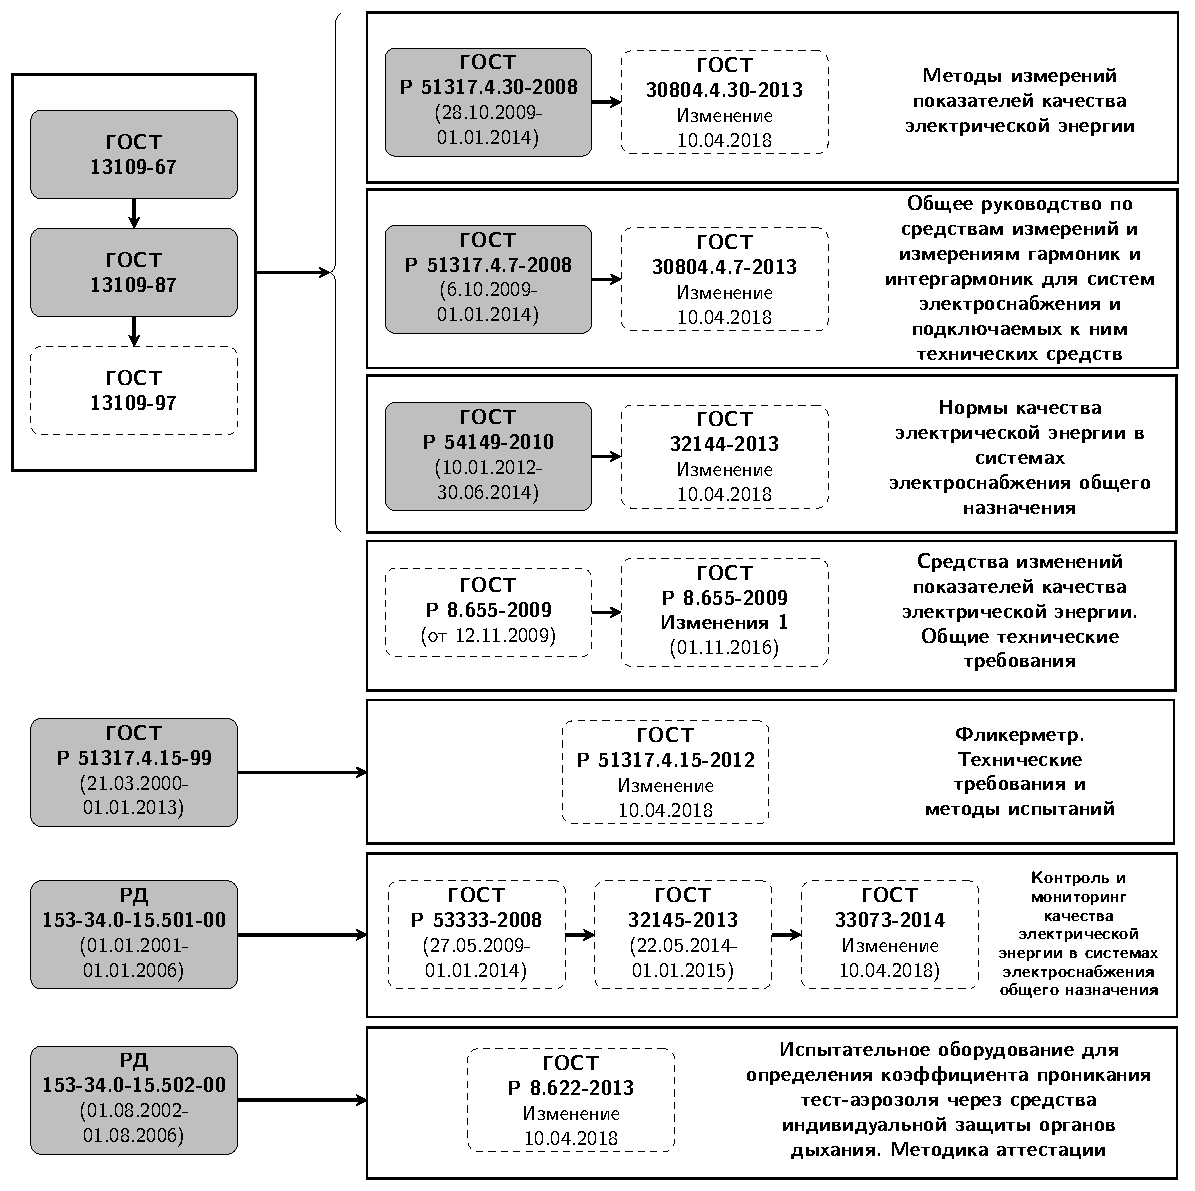
\includegraphics[scale=0.8]{picture1}
	}
	\caption{Развитие государственных стандартов в области контроля КЭ.}\label{img:picture1}
\end{figure}
%Действующие стандарты на рисунке

% [179 - ГОСТ 30804.4.30-2013 (IEC 61000-4-30:2008) Электрическая энергия. Совместимость технических средств электромагнитная. Методы измерений показателей качества электрической энергии (с Поправкой) [Электронный ресурс] / Режим доступа: http://docs.cntd.ru/document/1200104665]

% [4 - ГОСТ 30804.4.7-2013 (IEC 61000-4-7:2009) Совместимость технических средств электромагнитная. Общее руководство по средствам измерений и измерениям гармоник и интергармоник для систем электроснабжения и подключаемых к ним технических средств (с Поправкой) [Электронный ресурс] / Режим доступа: http://docs.cntd.ru/document/1200103652]

% [125 - ГОСТ 32144-2013 Электрическая энергия. Совместимость технических средств электромагнитная. Нормы качества электрической энергии в системах электроснабжения общего назначения [Электронный ресурс] – Режим доступа: http://docs.cntd.ru/document/1200104301/]

% [136 - ГОСТ Р 8.655-2009 Государственная система обеспечения единства измерений (ГСИ). Средства измерений показателей качества электрической энергии. Общие технические требования (с Изменением N 1) [Электронный ресурс] / Режим доступа: http://docs.cntd.ru/document/1200075494/]

% [194 - ГОСТ Р 51317.4.15-2012 (МЭК 61000-4-15:2010) Совместимость технических средств электромагнитная. Фликерметр. Функциональные и конструктивные требования [Электронный ресурс] / Режим доступа: http://docs.cntd.ru/document/1200096463]

% [195 - ГОСТ 33073-2014 Электрическая энергия. Совместимость технических средств электромагнитная. Контроль и мониторинг качества электрической энергии в системах электроснабжения общего назначения (с Поправкой) [Электронный ресурс] / Режим доступа: http://docs.cntd.ru/document/1200115349]

% [196 - ГОСТ 8.622-2013 Государственная система обеспечения единства измерений (ГСИ). Испытательное оборудование для определения коэффициента проникания тест-аэрозоля через средства индивидуальной защиты органов дыхания. Методика аттестации [Электронный ресурс] / Режим доступа: http://docs.cntd.ru/document/1200108162]

Основополагающим нормативным документом в Российской Федерации, регламентирующим положения связанные с КЭ в Российской Федерации, был ГОСТ~13109--97 \cite{GOST13109-97}. 

Стандарт не отвечал современным реалиям и заменен на ГОСТ~32144--2013 \cite{GOST32144-2013}, действует с 01.07.2014~г. приказом Росстандарта. Российский стандарт соответствует европейскому ЕN 50160:2010 <<Характеристики напряжения электричества, поставляемого общественными распределительными сетями>> \cite{ЕN50160:2010}. Действующий зарубежный стандарт DIN~EN~50160--2011 \cite{DINEN50160-2011}. DIN (Deutsches Institut für Normung – немецкий институт по стандартизации) – государственный стандарт Германии. EN (EuroNorm) – европейский стандарт, принятый Европейским комитетом по стандартизации CEN (European Committee for Standardization).

% [11 - 11.	EN 50160:2010 Voltage characteristics of electricity supplied by public electricity networks [Электронный ресурс] / Режим доступа: https://infostore.saiglobal.com/preview/98699522296.pdf?sku=859794_saig_nsai_nsai_2045468]

Новый стандарт ГОСТ~32144--2013 по требованиям к КЭ учитывает рекомендации положений международных стандартов и новых национальных стандартов по методам и средствам измерения и оценки ПКЭ, а также сближает структуру и положения данного стандарта с европейским стандартом ЕN~50160:2010.
Определение понятия средства измерений (СИ) в ГОСТ~30804.4.7--2013 \cite{GOST30804.4.7-2013}.
СИ предназначенных для, измерений спектральных составляющих напряжения и тока в полосе частот до 9 кГц, которые наложены на основные составляющие в системах электроснабжения частотой 50 и 60 Гц.


Некоторые принципиальные отличия  ГОСТ~32144--2013 \cite{GOST32144-2013} от предыдущего стандарта ГОСТ~13109--97 \cite{GOST13109-97}: 
%\noindent Маркированный список:
\begin{itemize}
	\item Отличие по интервалам усреднения показателям качества электроэнергии (отклонение частоты -- 10~сек., вместо 20~сек. в ГОСТ~13109--97; не симметрия напряжения -- интервал усреднения 10~мин., вместо 3~сек. в ГОСТ~13109--97; гармонические составляющие напряжения -- 10~мин., вместо 3~сек. в ГОСТ~13109--97) с интервалом периода в одну неделю, вместо суток в ГОСТ~13109--97.
	\item Измерения согласно ГОСТ~30804.4.30--2013 (IEC~61000--4--30:2008) \cite{GOST30804.4.30-2013} и ГОСТ~30804.4.7–-2013 (IEC~61000--4--7:2009) \cite{GOST30804.4.7-2013}.
	\item Для медленных изменений напряжения исключены режимы наименьших и наибольших нагрузок.
	\item Добавлены таблицы классификации провалов напряжения по остаточному напряжению.
\end{itemize}

При невыполнении энергоснабжающей организации требований к ПКЭ (в соответствии с ГОСТ 32144-2013 \cite{GOST32144-2013}, обязательным к применению в соответствии с
частью 1 статьи 46 Федерального закона от 27.12.2002 № 184-ФЗ «О техническом регулировании») наступает административная ответственность по статье $14.43$
«Кодекса Российской Федерации об административных правонарушениях» \cite{Serkov2017Problems} %c. 53.

Кроме Российских стандартов, существуют Международные регламентирующие документы по мониторингу КЭ, рекомендация от Института инженеров электротехники (IEEE -- Institute of Electrical and Electronics Engineers) \cite{IEEE_PES}. На рисунке \ref{img:picture2} изображен логотип IEEE.
% [12 -	IEEE PES Power Quality Subcommittee [Электронный ресурс] / Режим доступа: https://site.ieee.org/pes-pq/]

\begin{figure}[ht]
	\centering
	
\includegraphics [scale=0.5] {Logo_IEEE.png}
	\caption{Логотип института инженеров электротехники и электроники.}
	\label{img:picture2}
\end{figure}

IEEE PES Power Quality Subcommittee (IEEE PES по качеству электроэнергии) участвует в качестве представителя Национального комитета США в Международной конференции и выставке по распределению электроэнергии (CIRED -- Congres International des Reseaux Electriques de Distribution) \cite{CIRED, CIRED_CONFERENCE}. 
% [197 - INTERNATIONAL CONFERENCE ON ELECTRICITY DISTRIBUTION  [Электронный ресурс] / Режим доступа: http://www.cired.net/]

%[198 - THE 25TH INTERNATIONAL CONFERENCE AND EXHIBITION ON ELECTRICITY DISTRIBUTION [Электронный ресурс] / Режим доступа: http://www.cired2019.org/page/about-cired]

Группа международных стандартов в области контроля КЭ:
\begin{itemize}
	\item Стандарт IEEE~519--2014: рекомендуемая практика и требования IEEE для гармонического управления в электроэнергетических системах (IEEE~519--2014 -- IEEE Recommended Practice and Requirements for Harmonic Control in Electric Power Systems)\cite{IEEE_519-2014}. 
	\item Стандарт IEEE~1159--2019: рекомендуемая практика IEEE для мониторинга качества электроэнергии (1159--2019 -- IEEE Recommended Practice for Monitoring Electric Power Quality) \cite{IEEE_1159-2019}. 
	\item Стандарт 1159.3--2019: рекомендуемая практика IEEE для формата обмена данными о качестве электроэнергии (1159.3--2019 -- IEEE Recommended Practice for Power Quality Data Interchange Format (PQDIF)\cite{IEEE_1159.3-2019}.
	\item Стандарт IEEE~1250-2018 -- Руководство IEEE по выявлению и улучшению качества напряжения в энергосистемах (IEEE~1250--2018 -- IEEE Guide for Identifying and Improving Voltage Quality in Power Systems)\cite{IEEE_1250-2018}.
	\item Стандарт IEEE~1409--2012 -- Руководство IEEE по применению силовой электроники для повышения качества электроэнергии в распределительных системах. Номинальные значения: от 1 до 38~кВ. (IEEE~1409--2012 -- IEEE Guide for Application of Power Electronics for Power Quality Improvement on Distribution Systems Rated 1~kV Through 38~kV)\cite{IEEE_1409-2012}.
	\item Стандарт IEEE~1453-2015: рекомендуемая практика IEEE для анализа колеблющихся установок в энергосистемах (IEEE~1453--2015 -- IEEE Recommended Practice for the Analysis of Fluctuating Installations on Power Systems).
	\item Стандарт IEEE~1564--2014 -- Руководство IEEE по показателям падения напряжения (IEEE~1564--2014 -- IEEE Guide for Voltage Sag Indices) \cite{IEEE_1453-2015}.
\end{itemize}

Группа международных стандартов описывает факторы, влияющие на КЭ \cite{IEEE_519-2014, IEEE_1159-2019, IEEE_1159.3-2019, IEEE_1250-2018, IEEE_1564-2014, IEEE_1409-2012, IEEE_1453-2015, IEEE_1159-2009}:

\begin{itemize}
	\item IEC~61000--4--30:~2015 -- Электромагнитная совместимость. Часть 4-30. Методы испытаний и измерений. Методы измерения качества электроэнергии (Electromagnetic compatibility (EMC) -- Part~4-30: Testing and measurement techniques - Power quality measurement methods) \cite{IEC61000-4-30:2015}.
	\item IEC~TR~61000--1--1:~1992 -- Электромагнитная совместимость. Часть~1. Общие положения. Раздел~1. Применение и толкование основных определений и терминов (Electromagnetic compatibility (EMC) -- Part~1: General -- Section 1: Application and interpretation of fundamental definitions and terms) \cite{IEC_TR_61000-1-1:1992}.
	\item IEC~61000--1--2:~2016 -- Электромагнитная совместимость. Часть~1-2. Общие положения. Методология обеспечения функциональной безопасности электрических и электронных систем, включая оборудование в отношении электромагнитных явлений (Electromagnetic compatibility (EMC) -- Part~1-2: General -- Methodology for the achievement of functional safety of electrical and electronic systems including equipment with regard to electromagnetic phenomena) \cite{IEC61000-1-2:2016}.
	\item IEC~TR~61000--1--3:~2002 -- Электромагнитная совместимость (ЭМС). Часть~1-3. Общие положения. Воздействие высотной ЭМИ (HEMP) на гражданское оборудование и системы (Electromagnetic compatibility (EMC) -- Part~1-3: General -- The effects of high-altitude EMP (HEMP) on civil equipment and systems) \cite{IECTR61000-1-3:2002}.
\end{itemize}

%[200 - IEC 61000-4-30:2015 Electromagnetic compatibility (EMC) - Part 4-30: Testing and measurement techniques - Power quality measurement methods [Электронный ресурс] / Режим доступа: https://webstore.iec.ch/publication/21844#additionalinfo]

%[201 - IEC TR 61000-1-1:1992 Electromagnetic compatibility (EMC) - Part 1: General - Section 1: Application and interpretation of fundamental definitions and terms [Электронный ресурс] / Режим доступа: https://webstore.iec.ch/publication/4120] 

%[202 - IEC 61000-1-2:2016 Electromagnetic compatibility (EMC) - Part 1-2: General - Methodology for the achievement of functional safety of electrical and electronic systems including equipment with regard to electromagnetic phenomena [Электронный ресурс] / Режим доступа: https://webstore.iec.ch/publication/24517]

%[203 - IEC TR 61000-1-3:2002 Electromagnetic compatibility (EMC) - Part 1-3: General - The effects of high-altitude EMP (HEMP) on civil equipment and systems [Электронный ресурс] / Режим доступа: https://webstore.iec.ch/publication/4122]

Национальный комитет США Международной электротехнической комиссии (USNC/IEC) предоставляет стратегию для эффективного участия в разработке стандартов. USNC участвует почти во всей технической программе Международной электротехнической комиссии (МЭК) и управляет многими ключевыми комитетами и подгруппами 	\ref{img:picture3}.

\begin{figure}[ht]
	\centering
	
\includegraphics [scale=1] {Logo_IEC.jpg}
	\caption{Логотип международной электротехнической комиссии.}
	\label{img:picture3}
\end{figure}


IEC является ведущей глобальной организацией, которая готовит и публикует международные стандарты для электрических, электронных и смежных технологий. Они служат основой для национальной стандартизации и справочными материалами при разработке международных тендеров и контрактов.
USNC/IEC является полностью интегрированным комитетом Американского национального института стандартов (ANSI -- American National Standards Institute, Incorporated). ANSI служит ключевым ресурсом для стандартов и информации \cite{ANSI}.
%[204 - American National Standards Institute [Электронный ресурс] / Режим доступа: https://www.ansi.org/standards_activities/iec_programs/overview]

Два российских стандарта были разработаны на основе стандартов Международной Электротехнической Комиссии (International Electrotechnical Commission) IEC 61000--4--30:2008 и IEC 61000--4--7--2002:
\begin{itemize}
	\item ГОСТ 30804.4.30--2013 (IEC 61000--4--30:2011) Методы измерений показателей качества электрической энергии \cite{GOST30804.4.30-2013}.
	\item ГОСТ 30804.4.7--2013 (IEC 61000--4--7:2011) Общее руководство по средствам измерений и измерениям гармоник и интергармоник для систем электроснабжения и подключаемых к ним технических средств \cite{GOST30804.4.7-2013}.
\end{itemize}

Стандарты, описывающие измерения параметров сети:
\begin{itemize}
	\item ГОСТ~30804.4.30 -- 2013 (PN~EN~61000--4--30:2011) -- Электромагнитная совместимость (EMC) -- Методы исследований и измерения – Метод измерения качества электроэнергии.
	\item ГОСТ~30804.4.7 -- 2013 (PN~EN~61000--4--7:2007) -- Электромагнитная совместимость (EMC) -- Методы исследований и измерений -- Общее руководство по измерению гармоник и интергармоник и применяемые для этой цели измерительные приборы для сети электропитания и подключенные к ним устройства. 
	\item ГОСТ~Р~51317.4.15--2012 (PN~EN~61000--4--15:2011) -- Электромагнитная совместимость (EMC) -- Методы исследований и измерений -- Измеритель мерцания света (фликера) -- Функциональная и проектная спецификация.
	ГОСТ 32144--2013 (PN~EN~50160:2010) -- Нормы качества электрической энергии в системах электроснабжения общего назначения.
\end{itemize}

\section{Показатели качества электроэнергии, характеризующие несинусоидальность напряжения} \label{sec:ch4/sect2} 

К проблемам качества электрической энергии (КЭ) относится множество явлений. Различные причины способствуют на улучшение КЭ и характеристик оборудования \cite{GOST13109-97}.

В таблице \ref{tbl:test1} показаны: показатель качества электрической энергии (ПКЭ), свойства электрической энергии (ЭЭ) и виновники ухудщения качества электрической энергии (КЭ):
%Таблица 1
\begin{table} [p]%
	\caption{Свойства ЭЭ, ПКЭ, виновники ухудшения КЭ}%
	\label{tbl:test1}% label всегда желательно идти после caption
	\begin{SingleSpace}
		\setlength\extrarowheight{6pt} %вот этим управляем расстоянием между рядами, \arraystretch даёт неудачный результат
		\setlength{\tymin}{1.9cm}% минимальная ширина столбца
		\begin{tabulary}{\textwidth}{@{}>{\zz}L >{\zz}C >{\zz}C @{}}% Вертикальные полосы не используются принципиально, как и лишние горизонтальные (допускается по ГОСТ 2.105 пункт 4.4.5) % @{} позволяет прижиматься к краям
			\toprule     %%% верхняя линейка
			Показатель КЭ & 
			Свойства ЭЭ &
			Виновники ухудшения КЭ \\
			\midrule %%% тонкий разделитель. Отделяет названия столбцов. Обязателен по ГОСТ 2.105 пункт 4.4.5 
			Установившееся отклонение напряжения ${\delta U_y}$ &
			Отклонение напряжения &
			Энергоснабжающая организация \\
			
			Размах изменения напряжения~${\delta U_t}$ 
			
			Доза фликера ${P_t}$ &
			Колебания напряжения &
			Потребитель с переменной нагрузкой \\
			
			Коэффициент искажения синусоидальности кривой напряжения ${K_U}$ &
			Несинусоидальность напряжения &
			Потребитель с нелинейной нагрузкой \\
			
			Коэффициент $n$-oй гармонической составляющей напряжения ${K_{U(n)}}$ &
			Несинусоидальность напряжения &
			Потребитель с нелинейной нагрузкой \\
			
			Коэффициент несимметрии напряжений по обратной последовательности ${K_{2U}}$ &
			Несимметрия трехфазной системы напряжений &
			Потребитель с несимметричной нагрузкой \\
			
			Коэффициент несимметрии напряжений по нулевой последовательности ${K_{0U}}$ &
			Несимметрия трехфазной системы напряжений &
			Потребитель с несимметричной нагрузкой \\
			
			Отклонение частоты ${\Delta f}$ &
			Отклонение частоты &
			Энергоснабжающая организация \\
			
			Длительность провала напряжения ${\Delta t_p}$ & % Нужно вставить русский символ в формулу ∆t_п
			Провал напряжения &
			Энергоснабжающая организация \\
			
			Импульсное напряжение ${U_{imp}}$ &
			Импульс напряжения &
			Энергоснабжающая организация \\
			
			Коэффициент временного перенапряжения ${K_{per U}}$ &
			Временное перенапряжение &
			Энергоснабжающая организация \\
			
			\bottomrule %%% нижняя линейка
		\end{tabulary}%
	\end{SingleSpace}
\end{table}

Отклонение напряжение -- это отличие фактического напряжения работы систем электроснабжения от его номинального значения. Отклонение напряжения происходит под воздействием медленного изменения нагрузки в той или иной точке сети. 

Это отрицательно влияет на качество и срок службы бытовой электроприборов. Отклонение напряжение влияет на работу электросварочных машин. Так для точечной сварки отклонение напряжения на 15~\% приводит к браку продукции. Чрезмерное повышение напряжение приводит к росту нагрузки тока и мощности короткого замыкания. Для приборов с электрическими схемами реальную опасность представляет перегрев, сбой элементов схемы управления. Если элементы находятся, включены длительное время, то может произойти выход из строя элементов и прибор перестанет выполнять заложенные в него функции.



Причиной снижения качества электрической энергии на крупных промышленных предприятиях является наличие в узлах нагрузок электроприемников с нелинейными воль-амперными характеристиками. \cite{Accounting_Higher_harmonics_Plans_2013, Modeling_Questions_Lyutarevich2013}
Такие электроприемники потребляют ток, по форме отличающийся от синусоидального. 

В диссиртационной работе рассматривается оценка ПКЭ, характеризующая несинусоидальность напряжения. В ГОСТ 32144--2013 \cite{GOST32144-2013}, п. 4.2.4 Несинусоидальность напряжения -- обозначает искажение синусоидальной формы кривой напряжения.

Гармонические составляющие напряжения обусловлены нелинейными нагрузками электрических сетей, которые подключаются к сетям различного напряжения. 

Гармонические токи, полные сопротивления электрических сетей, напряжения гармонических составляющих в точках передачи ЭЭ изменяются во времени.

Если нагрузка в системе линейная, то и токи во всех ветвях синусоидальны. Наличие нелинейной нагрузки приводит к возникновению несинусоидальных токов во всех ветвях электрической сети, что приводит к возникновению несинусоидальной кривой напряжения во всех точках сети, что отрицательно влияет на работу электрической сети (рисунок \ref{img:picture4}). 

\begin{figure}[ht]
	\centering
	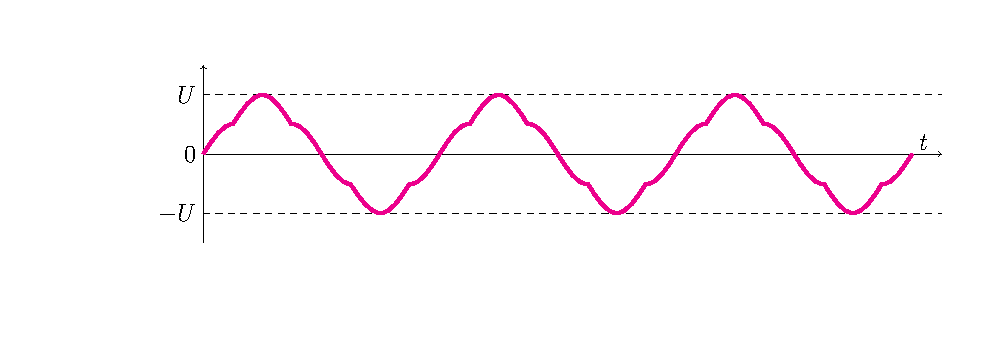
\includegraphics [scale=0.9] {non-sinusoidal_voltage}
	\caption{Несинусоидальность напряжения.}
	\label{img:picture4}
\end{figure}
Несинусоидальность напряжения характеризуется (ГОСТ 13109-97):
\begin{itemize}
	\item Коэффициентом искажения синусоидальности кривой напряжения.
	\item Коэффициентом $n$-ой гармонической составляющей напряжения.
\end{itemize} 

Импульс напряжения характеризуется показателем импульсного напряжения (рисунок \ref{img:picture5}).

\begin{figure}[ht]
	\centering
	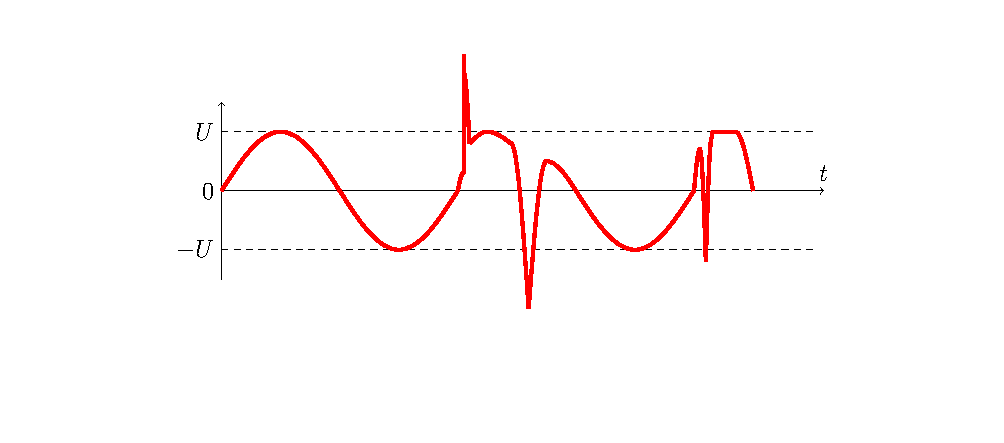
\includegraphics [scale=0.9] {voltage_pulses}
	\caption{Импульсы напряжения.}
	\label{img:picture5}
\end{figure}

На рисунке \ref{img:picture6}
изображены различные фрагменты напряжения. Провал напряжения (Voltagedip) характеризуется показателем длительности провала напряжения:
\begin{itemize}
	\item Предельно допустимое значение длительности провала напряжения в электрических сетях напряжения до $20$ кВ равно $30$ c.
	\item Данные характеризующие провалы напряжения в электрических сетях России напряжения $6-10$ кВ аналогичны данным в Европейских странах.
\end{itemize} 

Временное перенапряжение -- повышение напряжение электрической сети выше $1,1 U_{nom}$ продолжительностью больше $10$ мс, возникающее в системах электроснабжения при коммутациях или коротких замыканиях.

\begin{figure}[ht]
	\centering
	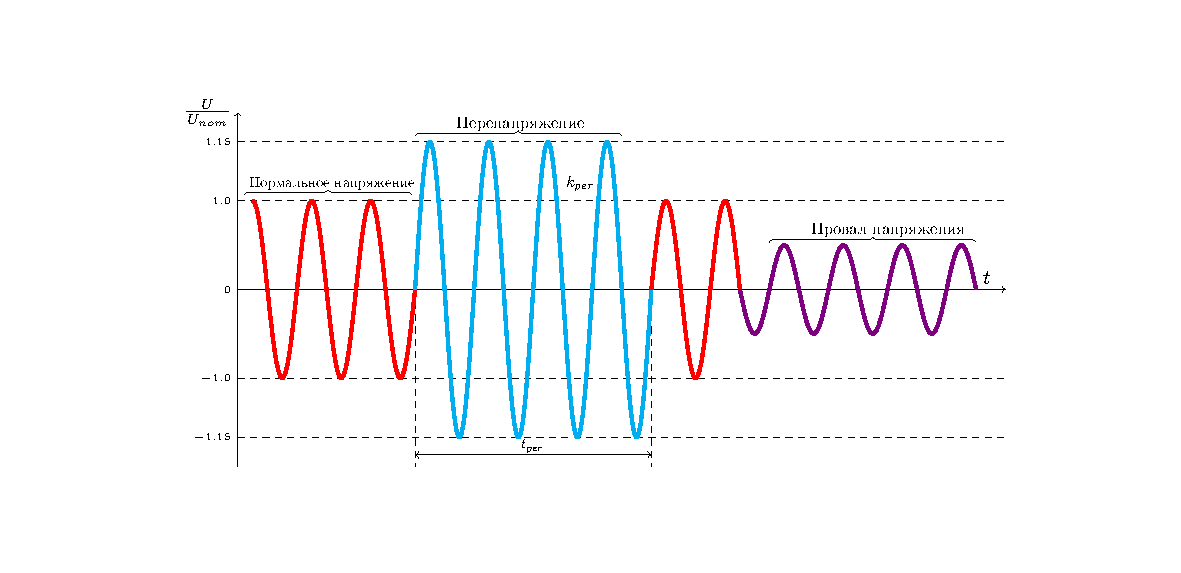
\includegraphics [scale=1.2] {voltagedip_overexertion}
	\caption{Фрагменты нормального напряжения в сети, перенапряжения и провала напряжения.}
	\label{img:picture6}
\end{figure}


% Нужен ли рисунок Несинусоидальность напряжения?
%график несинусоидального напряжения, если функция:
%plot(U(t) = 10*(sin(314*t) - (1/9)*sin(3*314*t) ) + (1/25)*sin(5*314*t) - (1/49)*sin(7*314*t)) В)
%https://www.wolframalpha.com/input/?i=plot%28U%28t%29+%3D+10*%28sin%28314*t%29+-+%281%2F9%29*sin%283*314*t%29+%29+%2B+%281%2F25%29*sin%285*314*t%29+-+%281%2F49%29*sin%287*314*t%29%29+%D0%92%29

%график несинусоидального тока, если функция:
%plot(I(t) = 10*(sin(314*t) + (1/3)*sin(3*314*t) )+(1/5)*sin(5*314*t)+(1/7)*sin(7*314*t)) А)
%https://www.wolframalpha.com/input/?i=plot%28I%28t%29+%3D+10*%28sin%28314*t%29+%2B+%281%2F3%29*sin%283*314*t%29+%29%2B%281%2F5%29*sin%285*314*t%29%2B%281%2F7%29*sin%287*314*t%29%29+%D0%90%29

%график несинусоидального тока, если функция:
%plot(I(t) = 10*(sin(314*t) + sin(350*t) ) А)
%https://www.wolframalpha.com/input/?i=plot%28I%28t%29+%3D+10*%28sin%28314*t%29+%2B+sin%28350*t%29+%29+%D0%90%29

Нелинейные и коммутируемые нагрузки могут вызвать искажения нормальных синусоидальных сигналов тока и напряжения в системе переменного тока. Источники искажений: силовые трансформаторы, преобразовательные устройства переменного тока.

Анализ несинусоидальности напряжения является составной частью системы эксплуатационного контроля КЭ. Для этого на шинах управления соответствующих контрольных пунктов устанавливают анализаторы несинусоидальности, которые соединены с регистрирующими приборами. Разлагают на спектральные составляющие, чтобы проанализировать несинусоидальность режимов напряжения. Поэтому, для повышения точности измерения показателей несинусоидальности напряжения необходимо повышать точность оценки гармонических и интергармонических составляющих напряжения. 

Существуют различия между утратившим силу стандартом ГОСТ 13109--97 \cite{GOST13109-97} и действующим ГОСТ 32144--2013 \cite{GOST32144-2013}.

Сравнительный анализ стандартов качества электрической энергии ГОСТ 13109--97 и ГОСТ 32144--2013 \cite[с.~155]{Comparative_analysis_Kiselev_2016}
% [205 - Киселёв Б. Ю. Сравнительный анализ стандартов качества электрической энергии ГОСТ 13109–97 и ГОСТ 32144–2013 // Молодой ученый. — 2016. — №20. — С. 155-157. — URL https://moluch.ru/archive/124/34114/ (дата обращения: 09.10.2019)]

Основные отличия в ГОСТ 32144-2013:
\begin{itemize}
	\item Изменен интервал времени, соответствующий расчетному интервалу времени на одну неделю.
	\item Изменения характеристик ЭЭ разделены на две категории – продолжительные изменения характеристик напряжения и случайные события.
	\item Процедура проведения контроля производится на основе ГОСТ Р~51317.4.30--2008 \cite{GOSTR51317.4.30-2008} и ГОСТ~Р~51317.4.7--2008 \cite{GOSTR51317.4.7-2008}.
	\item Введены интергармонические составляющие напряжения, хотя ни каких ограничений по их отклонению пока нет, они находятся на стадии разработки.
	\item Вместо коэффициента искажения синусоидальности кривой напряжения несинусоидальность напряжения характеризуется суммарным коэффициентом гармонических составляющих.
\end{itemize} 

% ГОСТ Р 51317.4.30-2008 (Недействующий) -> ГОСТ 30804.4.30-2013 (Действующий)
% [3 - ГОСТ Р 51317.4.30-2008 (МЭК 61000-4-30:2008). Совместимость технических средств электромагнитная. Методы измерений показателей качества электрической энергии [Электронный ресурс] – Режим доступа: http://docs.cntd.ru/document/1200072576]
% [179 - ГОСТ 30804.4.30–2013 (IEC 61000-4-30:2008) Электрическая энергия. Совместимость технических средств электромагнитная. Методы измерений показателей качества электрической энергии [Электронный ресурс] – Режим доступа: http://docs.cntd.ru/document/1200104665]

% ГОСТ Р 51317.4.7–2008 (Недействующий) -> ГОСТ 30804.4.7-2013 (Действующий)
% [4 - ГОСТ 30804.4.7-2013 (IEC 61000-4-7:2009) Совместимость технических средств электромагнитная. Общее руководство по средствам измерений и измерениям гармоник и интергармоник для систем электроснабжения и подключаемых к ним технических средств.]

В ГОСТ 13109--97 \cite{GOST13109-97} коэффициент искажения синусоидальности кривой напряжения $K_U$ определен как \eqref{eq:$K_U$}:

\begin{equation}
	\label{eq:$K_U$}
	K_U = \frac{\sqrt{\sum_{n=2}^N {U_{(n)}}^2}}{U_{(1)}}\cdot 100 \%
\end{equation}


где $U_{(n)}$ -- Действующее значение $n$-ой гармонической составляющей напряжения;

$n$ -- Порядок гармонической составляющей напряжения;

$N$ -- Порядок последней из учитываемых гармонических составляющих напряжения (стандартом устанавливается $N=40$);

$U_{(1)}$ -- Действующее значение напряжения основной частоты.

Также допускается определять коэффициент искажения синусоидальности кривой напряжения $K_{U2}$ по следующему выражению \ref{eq:$K_U2$}:
\begin{equation}
	\label{eq:$K_U2$}
	K_U = \frac{\sqrt{\sum_{n=2}^N {U_{(n)}}^2}}{U_{nom}}\cdot 100 \%,
\end{equation}

где $U_{nom}$ -- Номинальное напряжение сети.

Коэффициент n-ой гармонической составляющей напряжения равен:

\begin{equation}
	\label{eq:$K_U(n)$}
	K_{U(n)} = \frac{U(n)}{U(1)} \cdot 100 \%.
\end{equation}

В связи с тем, что существует ряд явлений, которые влияют на напряжение, поэтому сложно установить определенные допустимые границы значений для соответствующих характеристик напряжения. Поэтому такие определения как -- провалы и прерывания напряжения, перенапряжение, импульсные напряжения в стандарте \cite{GOST32144-2013} не нормируются. 

Методы измерения показателей КЭ установлены в стандартах ГОСТ 30804.4.30--2013 \cite{GOST30804.4.30-2013} и ГОСТ 30804.4.7--2013 \cite{GOST30804.4.7-2013}   

Согласно ГОСТ 13109--97 нормально допустимые и предельно допустимые значения коэффициента искажения синусоидальности кривой напряжения в точке общего присоединения к электрическим сетям с разным номинальным напряжением приведены в таблице \ref{tbl:test2}. 

%Таблица 2
\begin{table}[ht]
	\caption{Значения коэффициента искажения синусоидальности кривой напряжения согласно ГОСТ 13109--97 (в процентах)}%
	\label{tbl:test2}%
	\fontsize{14pt}{14pt}\selectfont
	\begin{longtable*}[c]{|c|c|c|c|c|c|c|c|} 
		\hline
		\multicolumn{4}{|c|}{Нормально допустимые}  &		
		\multicolumn{4}{c|}{Предельно допустимые}  \\		
		
		\multicolumn{4}{|c|}{значения при $U_{nom}$, кВ}  &		
		\multicolumn{4}{c|}{значения при $U_{nom}$, кВ}  \\		
		
		\hline
		$0,38$ &
		$6-20$ &
		$35$ &
		$110-330$ &
		$0,38$ &
		$6-20$ &
		$35$ &
		$110-330$ \\
		
		\hline
		$8,0$ &
		$5,0$ &
		$4,0$ &
		$2,0$ &
		$12,0$ &
		$8,0$ &
		$6,0$ &
		$3,0$ \\
		\hline
	\end{longtable*}
\end{table}

В ГОСТ 32144--2013 \cite{GOST32144-2013} представлены таблицы \ref{tbl:test3}, \ref{tbl:test4} для суммарных коэффициентов гармонических составляющих напряжения $K_{U(n)}$.

%Таблица 3
\begin{table}[ht]%
	\caption{Значения суммарных коэффициентов гармонических составляющих напряжения $K_{U(n)}$ согласно ГОСТ 32144--2013.}%
	\label{tbl:test3}% label всегда желательно идти после caption
	\fontsize{14pt}{14pt}\selectfont
	\begin{longtable*}[c]{|c|c|c|c|}  
		\hline
		\multicolumn{4}{|c|}{Значения суммарных коэффициентов}  \\
		\multicolumn{4}{|c|}{гармонических составляющих напряжения} \\
		\multicolumn{4}{|c|}{$K_{U(n)}$ ,\%} \\
		\hline	
		\multicolumn{4}{|c|}{Напряжение электрической сети, кВ} \\			
		\hline			
		$0,38  $        &
		$6-25$          &
		$35$            &
		$110-220$ \\
		\hline
		$8,0$ &
		$5,0$ &
		$4,0$  &
		$2,0$ \\
		\hline
	\end{longtable*}%
\end{table}

В качестве суммарных коэфициентов гармонических составляющих напряжения $K_{U(n)}$ должны применены сумарные коэффициенты гармонических подгрупп по ГОСТ 30804.4.7, раздел 3.3 \cite{GOST30804.4.7-2013}.

%Таблица 4
\begin{table}[ht]%
	\caption{Значения суммарных коэффициентов гармонических составляющих напряжения $K_{U(n)}$ согласно ГОСТ 32144--2013.}%
	\label{tbl:test4}% label всегда желательно идти после caption
	\fontsize{14pt}{14pt}\selectfont
	\begin{longtable*}[c]{|c|c|c|c|}  
		\hline
		\multicolumn{4}{|c|}{Значения суммарных коэффициентов}  \\
		\multicolumn{4}{|c|}{гармонических составляющих напряжения} \\	
		\multicolumn{4}{|c|}{ $K_{U(n)}$ ,\% } \\	
		\hline
		\multicolumn{4}{|c|}{Напряжение электрической сети, кВ} \\			
		\hline			
		$0,38$ &
		$6-25$ &
		$35$  &
		$110-220$ \\
		\hline			
		$12,0$ &
		$8,0$ &
		$6,0$  &
		$3,0$ \\
		\hline
	\end{longtable*}%
\end{table}


Суммарный коэффициент гармонических составляющих (total harmonic distortion, THD) -- это отношение среднеквадратичного значения суммы всех гармонических составляющих $Y_{H,h}$ до порядка $h_{max}$ к среднеквадратичному значению основной составляющей $Y_{H,1}$.

\begin{equation}
	\label{eq:$THD_Y$}
	THD_Y = \sqrt{\sum_{h=2}^{h_{max}}\left( \frac{Y_{H,h}}{Y_{H,1}}\right) ^2},
\end{equation}

где ${Y_{H,h}}$ -- Cреднеквадратичное значение гармонической составляющей порядка $h$.

$h$ -- Текущее целое число, обозначающее порядок гармоники.

${h_{max}}$ -- Порядок высшей учитываемой гармонической составляющей.  

Максимальное значение принимают равным 40, если иное не установлено международных стандартах. Символ Y (переменная) может быть заменен на I (для тока), U (для напряжения). 

В ГОСТ 13109--97 термин <<коэффициент искажения синусоидальности кривой напряжения>> $K_U$ обозначает суммарный коэффициент гармонических составляющих.

%Таблица 4
\begin{table}[ht]
	\caption{Значения коэффициентов нечетных гармонических составляющих напряжения не кратных трем (в процентах).}%
	\label{tbl:test5}%
	\fontsize{14pt}{14pt}\selectfont
	\begin{longtable*}[c]{|c|c|c|c|c|} %longtable* появляется из 
		\hline
		Порядок & 
		\multicolumn{4}{l|}{Значения коэффициентов гармонических}  \\
		гармонической &
		\multicolumn{4}{l|}{составляющих напряжения $K_{U(n)}$ ,\% ${U_1}$}\\		
		составляющей&
		\multicolumn{4}{l|}{Напряжение электрической сети, кВ} \\			
		\hline
		$n$&
		$0,38$ кВ &
		$6-25$~кВ &
		$35$ кВ  &
		$110-220$~кВ \\
		
		\hline
		
		$5$ &
		$6$ &
		$4$ &
		$3$ &
		$1,5$ \\
		
		$7$ &
		$5$ &
		$3$ &
		$2,5$&
		$1$ \\
		
		$11$ &
		$3,5$ &
		$2$ &
		$2$ &
		$1$ \\
		
		$13$ &
		$3,0$ &
		$2$ &
		$1,5$ &
		$0,7$\\
		
		$17$ &
		$2,0$ &
		$1,5$ &
		$1$ &
		$0,5$\\
		
		$19$ &
		$1,5$ &
		$1$	&
		$1$ &
		$0,4$\\
		
		$23$ &
		$1,5$ &
		$1$ &
		$1$ &
		$0,4$\\
		
		$25$ &
		$1,5$ &
		$1$ &
		$1$ &
		$0,4$\\
		
		$>25$ &
		$1,5$ &
		$1$ &
		$1$ &
		$0,4$\\
		\hline
	\end{longtable*}
\end{table}



%Таблица 5
\begin{table} [ht]%
	\caption{Значения коэффициентов нечетных гармонических  составляющих напряжения кратных трем.}%
	\label{tbl:test5}% label всегда желательно идти после caption
	\fontsize{14pt}{14pt}\selectfont
	\begin{longtable*}[c]{|c|c|c|c|c|}  
		\hline
		Порядок & 
		\multicolumn{4}{|l|}{Значения коэффициентов гармонических}  \\
		
		гармонической &
		\multicolumn{4}{|l|}{составляющих напряжения $K_{U(n)}$ ,\% ${U_1}$}\\		
		
		составляющей &
		\multicolumn{4}{|l|}{Напряжение электрической сети, кВ} \\			
		
		\hline
		$n$ &
		
		$0,38$ кВ &
		$6-25$~кВ &
		$35$ кВ  &
		$110-220$~кВ \\
		\hline
		$3$ &
		$5$ &
		$3$ &
		$3$ &
		$1,5$ \\
		
		$9$ &
		$1,5$ &
		$1$ &
		$1$&
		$0,4$ \\
		
		$15$ &
		$0,3$ &
		$0,3$ &
		$0,3$ &
		$0,2$ \\
		
		$21$ &
		$0,2$ &
		$0,2$ &
		$0,2$ &
		$0,2$\\
		
		
		$>21$ &
		$0,2$ &
		$0,2$ &
		$0,2$ &
		$0,2$\\
		
		\hline			
	\end{longtable*}
\end{table}



%Таблица 6
\begin{table}[ht]%
	\caption{Значения нечетных гармонических составляющих напряжения.}%
	\label{tbl:test6}% label всегда желательно идти после caption
	\fontsize{14pt}{14pt}\selectfont
	\begin{longtable*}[c]{|c|c|c|c|c|}  
		\hline
		Порядок & 
		\multicolumn{4}{|l|}{Значения коэффициентов гармонических}  \\
		гармонической &
		\multicolumn{4}{|l|}{составляющих напряжения $K_{U(n)}$ ,\% ${U_1}$}\\		
		составляющей &
		\multicolumn{4}{|l|}{Напряжение электрической сети, кВ} \\			
		
		\hline
		$n$	&
		
		$0,38$ кВ &
		$6-25$~кВ &
		$35$ кВ  &
		$110-220$~кВ \\
		\hline
		$2$ &
		$2$ &
		$1,5$ &
		$1$ &
		$0,5$ \\
		
		$4$ &
		$1$ &
		$0,7$ &
		$0,5$&
		$0,3$ \\
		
		$6$ &
		$0,5$ &
		$0,3$ &
		$0,3$ &
		$0,2$ \\
		
		$8$ &
		$0,5$ &
		$0,3$ &
		$0,3$ &
		$0,2$ \\
		
		$10$ &
		$0,5$ &
		$0,3$ &
		$0,3$ &
		$0,2$ \\
		
		$12$ &
		$0,2$ &
		$0,2$ &
		$0,2$ &
		$0,2$ \\
		
		$>12$ &
		$0,2$ &
		$0,2$ &
		$0,2$ &
		$0,2$\\
		
		\hline			
	\end{longtable*}
\end{table}

%Стандарты:
%\cite{GOST30804.4.7-2013}
%\cite{GOST30804.4.30-2013}
%\cite{GOST33073-2014}
%\cite{GOST32144-2013}
%\cite{GOSTR54149-2010}
%\cite{GOSTR51317.4.30-2008}
%\cite{GOSTR51317.4.7-2008}
%\cite{GOST_R8.655-2009}
%\cite{GOST13109-97}
%\cite{GOST13109-87}
%\cite{GOST8.216-88}
%\cite{GOST19431-84}
%\cite{GOST12.3.019-80}
%\cite{GOST21027-75}
%\cite{GOST16263-70}
%\cite{GOST13109-67}
%\cite{GOSTR51317.4.15-2012}
%\cite{GOST8.622-2013}

\section{Обзор приборов контроля показателей КЭ} \label{sec:ch4/sect3} 
Показатель качества электрической энергии (ПКЭ) -- это величина, которая характеризует КЭ по одному или нескольким показателям. Определение термина в \cite{GOST33073-2014}, раздел 3.4.
Контроль ПКЭ осуществляется в соответствии с нормативными документами: ГОСТ~32144--2013 \cite{GOST32144-2013},  ГОСТ~33073--2014 \cite{GOST33073-2014}, ГОСТ~30804.4.30--2013 \cite{GOST30804.4.30-2013}. 

Стандарты установлены при измерении ПКЭ в электрических сетях систем электроснабжения:
\begin{itemize}
	\item Общего назначения однофазного и трехфазного переменного тока с частотой 50~Гц, присоединенных к Единой энергетической системе.
	\item Изолированных систем электроснабжения общего назначения.
	\item Систем электроснабжения промышленных предприятий.
\end{itemize}

Согласно стандартам, установлены требования к характеристикам средств измерений (СИ) ПКЭ с помощью сертифицированных приборов. Приборы внесены в Государственный реестр СИ в разделе <<Сведения об утвержденных типах средств измерений>> по приказу Федерального агентства по метрологии и техническому регулированию от 20.08.2014 г. №1286.

К такому роду приборов относятся показывающие и регистрирующие частотомеры и вольтметры, анализаторы качества напряжения, анализаторы несинусоидальности, осциллографы, анализаторы несимметрии, регистраторы искажения формы кривой, электроанализаторы \cite{Quality_electricity_1975}.
%[60 - Левин М. С., Мурадян А. Е., Сырых Н. Н. Качество электроэнергии в сетях сельских районов. – Энергия, 1975.]

Средств измерений, типы которых утверждены Росстандартом: вольтметры, амперметры, системы автоматизированные измерительные, счетчики электрической энергии, комплексы аппаратно-программные, преобразователи измерительные и другие.

В настоящее время на рынке СИ ПКЭ представлено большое количество приборов российского и зарубежного производства. Зарубежные приборы удобны и надежны в эксплуатации, но они дороже отечественных аналогов.

Зарубежные торговые марки, которые присутствует длительный период на рынке: Anritsu (Япония), APPA Technology Corporation (Тайвань), Fluke Corporation (США), Good Will Instrument (Тайвань), HT-ITALIA (Италия), K\&H (Тайвань), National Instruments (США), PENDULUM (Швеция, Rohde\&Schwarz (Германия), МНИПИ (Белорусь).

Рассмотрим подробнее отечественные СИ:
\begin{enumerate}
	\item <<АКИП-4204/1>>, <<АКИП-4204/2>> (АО <<ПриСТ>>, г.~Москва).
	\item <<ПАРМА РК1.01>>, <<ПАРМА Т400 S>> (ООО <<Парма>>, г.~Санкт-Петербург).
	\item <<ПКЭ-А>> (<<НПП Mars-Energo>>, г.~Санкт-Петербург).
	\item <<Ресурс-UF2M-3Т52-5-100-1000>> (НПП <<Электротехника>>, г.~Пенза).
	\item <<НЕВА-ПА>> (НПФ <<Энергосоюз>>, г.~Санкт-Петербург).
	\item <<ЩМК96>> (ОАО <<Электроприбор>>, г.~Чебоксары).
	\item <<Прорыв-Т-А>> (НПП <<Прорыв>>, г.~Петрозаводск).
	\item Осциллограф АльфаТрек С7-324С (<<КОМЗ - ИЗМЕРЕНИЯ>>, г.~Москва).
\end{enumerate}

Акционерное общество <<Приборы, Сервис, Торговля>> \cite{prist}  является владельцем в России торговой марки <<АРРА>> и <<АКИП>>.
%[207.	АО «ПриСТ» [Электронный ресурс]. 2019. Режим доступа: https://prist.ru/about/]
АО <<ПриСТ>> существует на рынке с 1994 года.
Компания обеспечивает поставку СИ для электро, радио измерений,измерений параметров окружающей среды:
\begin{itemize}
	\item Осциллографы.
	\item Генераторы.
	\item Вольтметры.
	\item Частотомеры.
	\item Источники питания.
	\item Анализаторы качества электроэнергии.
	\item Мультиметры.
	\item Электроизмерительные клещи.
	\item Измерители температуры и влажности и др.
\end{itemize}

Компания заказывает у различных производителей Европы, Азии и Америки изготовление средств измерения. Изделия проходят анализ соответствия с требованием стандарта ISO-9000, а также российскими стандартами. ISO (International Organization for Standardization) -- Международная организация по стандартизации. Основной стандарт, к унификации с которым стремится большинство национальных стандартов. Средства измерения проходят на соответствие с ГОСТ Р. 

На рисунке \ref{fig:picture8} изображен анализатор спектра фирмы <<АКИП>>:

\begin{figure}[ht]
	\centerfloat{
		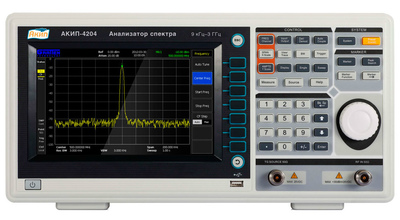
\includegraphics[scale=0.5]{AKIP}
	}
	\caption{<<АКИП>> 4204/1.}\label{fig:picture8}
\end{figure}

Анализаторы спектра фирмы АКИП предназначены для измерения амплитудно-частотных характеристик спектра радиотехнических сигналов. Серия анализаторов 4204 состоит из трех модификаций – 4204, 4204/1, 4204/2. Они отличаются верхней границей диапазона частот. Конструктивно анализаторы выполнены в виде настольного моноблока, объединяющие в своем составе высокочастотные и низкочастотные части и управляющий микропроцессор. Анализаторы работают под управлением встроенного микропроцессора. Они обеспечивают проведение автоматических измерений частотных и амплитудных параметров спектра сигналов. Полученные на приборах спектрограммы могут быть записаны в различных форматах во внутреннюю память, на внешний носитель, а также переданы на компьютер через интерфейс. 

% Таблица 7
\begin{table} [p]%
	\caption{Сравнительный анализ анализаторов спектра фирмы АКИП.}%
	\label{tbl:test7}% label всегда желательно идти после caption
	\begin{SingleSpace}
		\setlength\extrarowheight{6pt} %вот этим управляем расстоянием между рядами, \arraystretch даёт неудачный результат
		\setlength{\tymin}{1.7cm}% минимальная ширина столбца
		\begin{tabulary}{\textwidth}{@{}>{\zz}C >{\zz}C >{\zz}C >{\zz}C >{\zz}C >{\zz}C @{}}% Вертикальные полосы не используются принципиально, как и лишние горизонтальные (допускается по ГОСТ 2.105 пункт 4.4.5) % @{} позволяет прижиматься к краям
			\toprule     %%% верхняя линейка
			Параметры & \multicolumn{5}{c}{Торговая марка АКИП }  \\
			
			&
			$4205/2$ &
			$4204/2$ &
			$4204/1$ &
			$4204/1 TG$ &
			$4205/1 TG$ \\
			
			\midrule %%% тонкий разделитель. Отделяет названия столбцов. Обязателен по ГОСТ 2.105 пункт 4.4.5 
			
			Госреестр &
			Да &
			Да &
			Да &
			Да &
			Да \\
			
			Частотный диапазон &
			$9$~кГц - $3,2$~ГГц & 
			$9$~кГц - $7,5$~ГГц &
			$9$~кГц - $1,5$~ГГц &
			$9$~кГц - $1,5$~ГГц &
			$9$~кГц - $2,1$~ГГц \\
			
			Полоса пропускания (RBW) &
			$10$~Гц - $3$~МГц &
			$1$~Гц - $3$~МГц &
			$1$~Гц - $3$~МГц &
			$1$~Гц - $3$~МГц &
			$10$~Гц - $3$~МГц \\
			
			Полоса обзора &	
			$100$~Гц - $3,2$~ГГц &
			$100$~Гц - $3$~ГГц &
			$100$~Гц - $3$~ГГц &
			$100$~Гц - $1,5$ ГГц &
			$100$~Гц - $2,1$~ГГц \\
			
			Гармонические искажения &
			$-65$~дБн &
			$-70$~дБн &
			$-70$~дБн &
			$-70$~дБн &
			$-65$~дБн \\
			
			Уровень собственных шумов &
			$-146$~дБм &
			$-148$~дБм &
			$-148$~дБм &
			$-148$~дБм &
			$-146$~дБм \\
			
			Фазовый шум   &
			$-115$~дБн/Гц &
			$-95$~дБн/Гц  &
			$-100$~дБн/Гц &
			$-100$~дБн/Гц &
			$-115$~дБн/Гц \\
			
			Максимальный измеряемый уровень &	
			$20$~дБм &
			$30$~дБ  &
			$30$~дБ  &
			$30$~дБ  &
			$20$~дБм \\
			
			\bottomrule %%% нижняя линейка
		\end{tabulary}%
	\end{SingleSpace}
\end{table}

Компания <<Парма>> (ООО <<Парма>>, г.~Санкт-Петербург) занимается производством оборудования и систем для электроэнергетики: измерительные приборы, оборудование релейной защиты и автоматики, системы мониторинга переходных режимов, цифровые регистраторы аварийных процессов и другие приборы \cite{parma}. 
%[54 - Компания «ПАРМА» [Электронный ресурс]. 2018. Режим доступа: https://parma.spb.ru/company/about-company/.]

Регистратор качества электрической энергии ПАРМА РК1.01 \cite{parma2} в соответствии с требованиями ГОСТ 32144–2013 \cite{GOST32144-2013}. 
% Сайт прибора [https://parma.spb.ru/oborudovanie/registratory-kachestva-elektroenergii/]
Прибор малогабаритный, переносной для регистрации режимов однофазной сети $220$~В. Соответствии с классом S по ГОСТ 30804.4.30–2013 (IEC 61000–4–30:2008) \cite{GOST30804.4.30-2013}. Прибор используется для контроля качества электрической энергии, регистрации графиков нагрузок, а также расследование причин некорректной работы оборудования.
	
Измерительный преобразователь ПАРМА Т400 S \cite{parma1}.
	% Сайт прибора [https://parma.spb.ru/oborudovanie/mnogofunktsionalnye-izmeritelnye-preobrazovateli/]
Прибор предназначен для измерения параметров электрической энергии в сетях трехфазного и однофазного тока, а также преобразование информации в цифровой код. Передача данных происходит на микроконтроллер через последовательный интерфейс RS-485. Устройство нижнего уровня в Автоматизированных Информационно-измерительных Системах (АИИС) на объект генерации, передачи и распределения электроэнергии.

\begin{figure}[ht]
	\centerfloat{
		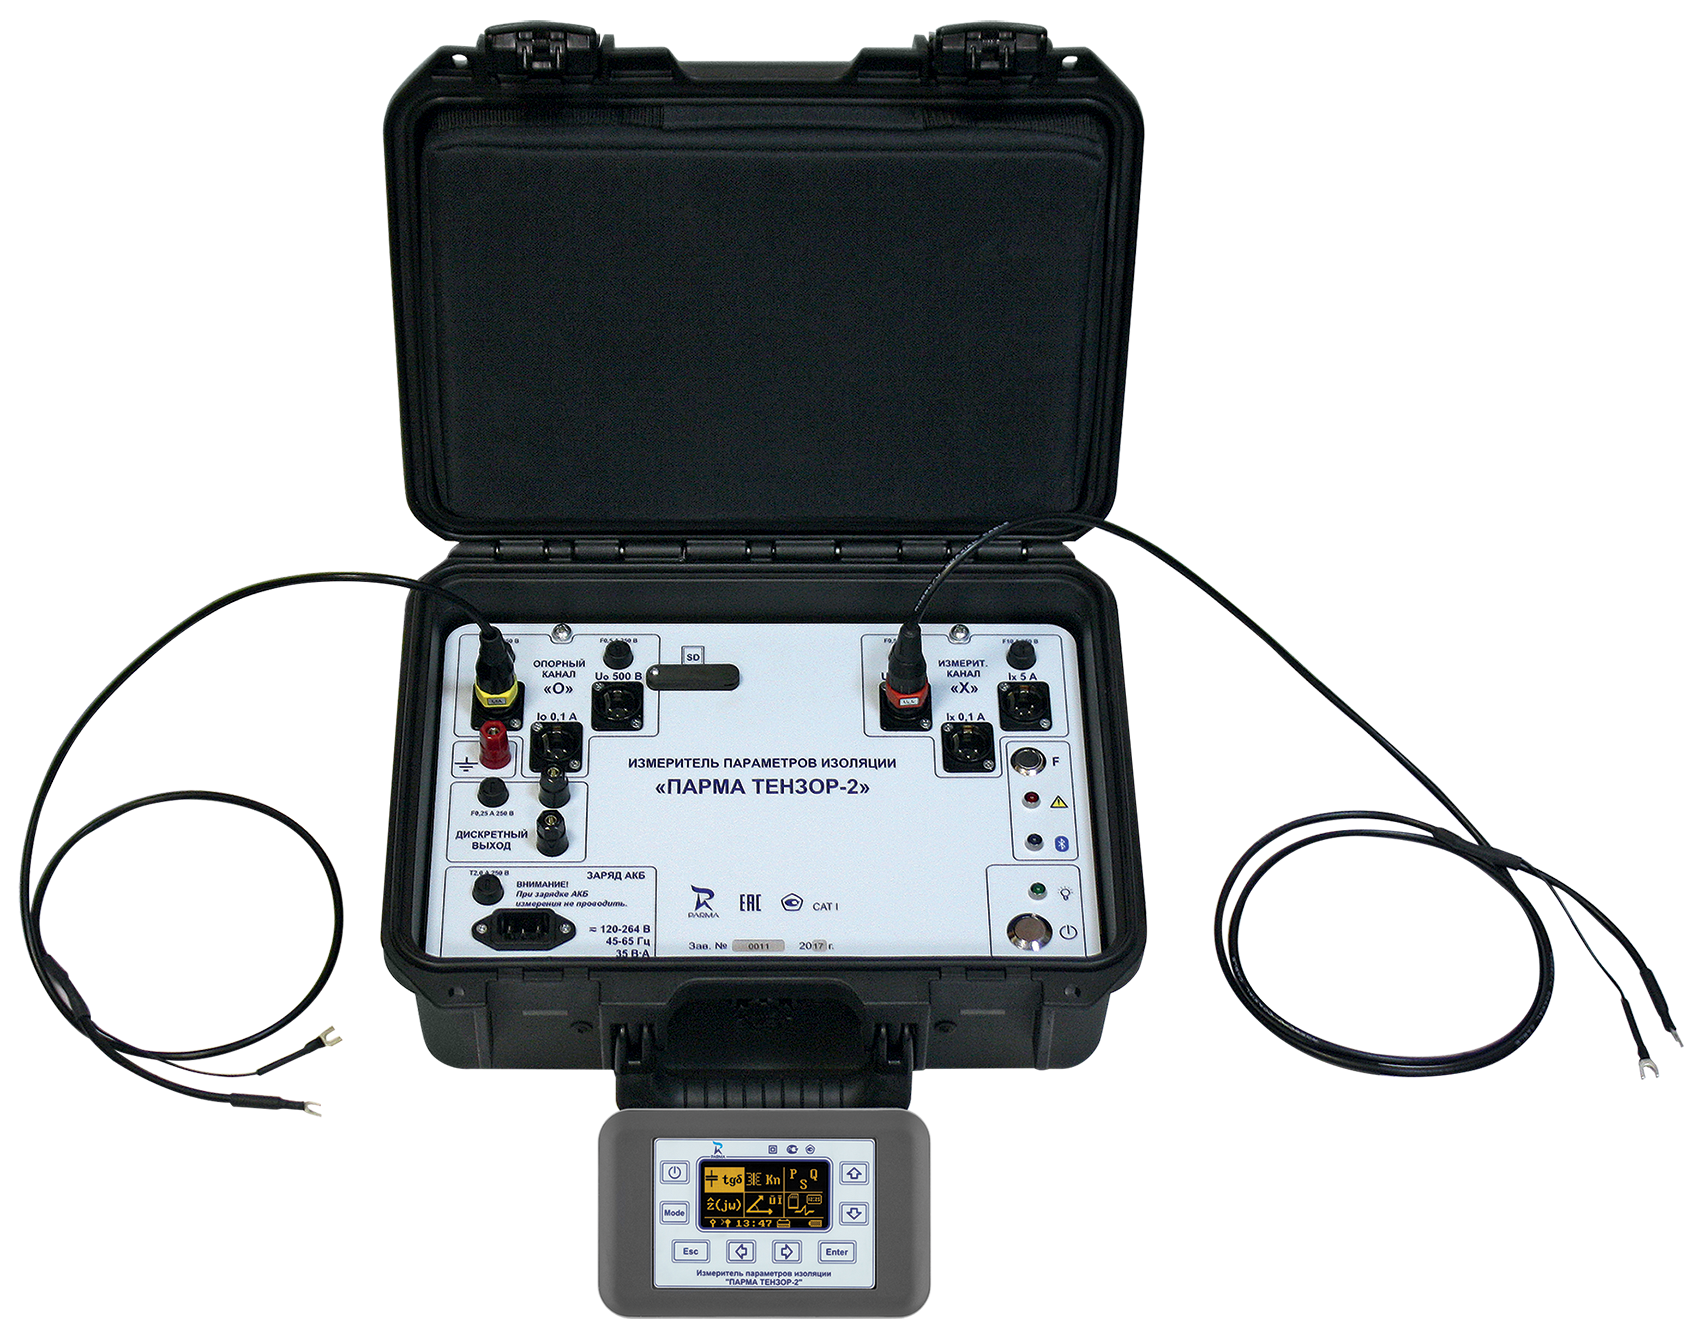
\includegraphics[scale=0.2]{parma_Tenzor}
	}
	\caption{<<ПАРМА>> Т400 S.}\label{fig:picture9}
\end{figure}

Компания Mars-Energo (НПП <<Mars-Energo>>, г.~Санкт-Петербург) изготавливает измерительные приборы, которые применяются на производственных предприятиях, в различных сферах электроэнергетики и органах Росстандарта. Компания существует в индустрии энергетики более 25~лет \cite{Mars-Energo}.
%[71 - «НПП Марс-Энерго» [Электронный ресурс]. 1999-2019. Режим доступа: http://www.mars-energo.ru/.]

Энерготестер ПКЭ-А прибор контроля качества электрической энергии \cite{energy_tester}.
% Ссылка на прибор [http://www.mars-energo.ru/home/pribory-kontrolya-kachestva-i-ucheta-elektroenergii/energotester-pke-a.html]
% Руководство эксплуатации [http://www.mars-energo.ru/home/pribory-kontrolya-kachestva-i-ucheta-elektroenergii/energotester-pke-a.html]
\begin{figure}[ht]
	\centerfloat{
		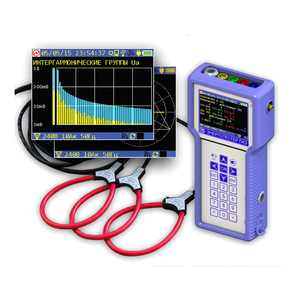
\includegraphics[scale=0.8]{ПКЭ-А}
	}
	\caption{Энерготестер ПКЭ-А.}\label{fig:picture10}
\end{figure}
Позволяет производить измерения в электросетях трех типов: трехфазной четырехпроводной, трехфазной трехпроводной и однофазной двухпроводной. Измерение и регистрация основных ПКЭ, установленных ГОСТ 32144--2013 \cite{GOST32144-2013} (ГОСТ Р 54149--2010) с оформлением протоколов по ГОСТ 33073--2014 \cite{GOST33073-2014}, в соответствии с ГОСТ 30804.4.30--2013 \cite{GOST30804.4.30-2013} (ГОСТ Р 51317.4.30--2008), ГОСТ 30804.4.7--2013 \cite{GOST30804.4.7-2013} (ГОСТ Р 51317.4.7--2008). 

Устройство позволяет проверять работоспособность и правильность подключения энергетических измерительных преобразователей напряжения, тока, активной и реактивной мощности на местах их эксплуатации. Измерения параметров вторичных цепей (мощности нагрузки) в системах учета электрической энергии. <<Энерготестер ПКЭ-А>>  проверяет работоспособность и правильность подключения однофазных и трехфазных счетчиков электрической энергии без разрыва токовых цепей.

\textbf{Научно-производственное предприятие <<Энерготехника>>}  (НПП <<Энерготехника>>, г.~Пенза) существует на рынке 26 лет. Основной изготавливаемой продукцией являются \cite{энерготехника}: 
%[73 - Научно-производственное предприятие «Энерготехника» [Электронный ресурс]. 2009-2019. Режим доступа: https://www.entp.ru/]

\begin{itemize}
	\item Измерители ПКЭ: <<Ресурс-UF2>>, <<Ресурс-UF2C>>, <<Ресурс-UF2М>>, <<Ресурс-ПКЭ>>.
	\item Счетчик многофункциональный <<Ресурс-Е4>>.
	\item Мультиметры: <<Ресурс-ПЭ>>, <<Ресурс-МТ>>.
	\item Калибраторы переменного тока <<Ресурс-К2>>,<<Ресурс-К2М>>.
\end{itemize}

Предприятие <<Энерготехника>> предоставляет измерение показателей качества электрической энергии, параметров напряжений, частоты, силы токов, активной и реактивной мощности, активной и реактивной энергии прямого и обратного направлений в трехфазных трехпроводных и четырехпроводных электрических сетях с помощью устройства система контроля качества электроэнергии <<Ресурс>> (СККЭ <<Ресурс>>). Устройство состоит из двух блоков: измерительного и  вычислительного.

<<Ресурс-UF2M-3Т52-5-100-1000>> измеритель показателей качества электрической энергии. Измерение ПКЭ производится согласно ГОСТ 30804.4.30--2013 \cite{GOST30804.4.30-2013} (ГОСТ Р 51317.4.30--2008), класс А, ГОСТ 32144--2013 \cite{GOST32144-2013} (ГОСТ Р 54149--2010). 

Прибор является мобильной версией прибора <<Ресурс‑UF2>>, обладает высокой точностью измерений силы тока без разрыва цепи с помощью токоизмерительных клещей (КТ52-5-100-1000 или КТ64-3000). Измеряет параметры напряжения, силы тока и угла фазового сдвига, мощности и энергии. <<Ресурс-UF2M-3Т52-5-100-1000>> записывает архивные данные на USB Flash-диск. Прибор регистрирует результаты измерений и аварийных событий, определяет выходную мощность измерительных трансформаторов напряжения, определяет погрешность счетчиков электрической энергии на месте эксплуатации. Прибор использует программное обеспечение: <<Ресурс-UF2 Opera>>, <<Ресурс-UF2 Plus>>, <<Ресурс-UF2 Plus>>, <<Монитор Ресурс-UF2>>, <<Ресурс-Бриз>>. 

ЗАО <<Научно-производственная фирма Энергосоюз>> (ЗАО <<НПФ Энергосоюз>>, г.~Санкт-Петербург)  c 1990 года специализируется на разработке, производстве и внедрении оборудования для автоматизации объектов электроэнергетики \cite{energy_union}.
% [69 - ЗАО «НПФ «ЭНЕРГОСОЮЗ» [Электронный ресурс]. 2009-2019. Режим доступа: http://www.energosoyuz.spb.ru/]

Один из первых разработок компании -- цифровой регистратор аварийных событий Блок Регистрации, Контроля и Управления (БРКУ), зарекомендовавший как надежное, функциональное и простое в работе устройство. Продукция компании: Регистраторы аварийных событий, Телемеханика, Противоаварийная автоматика, Контроль и диагностика, Автоматика управления, Измерительные приборы, Серверное оборудование, ПО <<СКАДА-НЕВА>>.
Устройство противоаварийной автоматики <<НЕВА-ПА>> \cite{neva-pa}. 
% Сайт прибора https://www.energosoyuz.spb.ru/ru/content/ustroystvo-protivoavariynoy-avtomatiki-neva-pa
Микропроцессорное устройство позволяет реализовать сложные алгоритмы противоаварийного управления: восстанавливать нормальное питание потребителей, выявлять и локализовать, развитие и аварийных режимов в энергосистемах, а также повышать пропускную способность электрических сетей. Основные функции устройства: предотвращать нарушение устойчивости, ликвидировать асинхронные режимы, ограничивать снижение или повышение частоты, ограничивать снижение или повышение напряжения, предотвращать перегрузку оборудования. Устройство <<НЕВА-ПА>> выполнено в блочном каркасе, имеет модульную структуру и снабжено для монтажа в несущую стоечную конструкцию типового шкафа управления.

Открытое акционерное общество (ОАО <<Электроприбор>>, г.~Чебоксары) – компания по производству щитовых аналоговых и цифровых электроизмерительных приборов, измерительныз преобразователей, приборов телемеханики, приборов для контроля ПКЭ. Основные напрвления компании: контрольно измерительные приборы и средства автоматизации.
<<ЩМК96>> прибор контроля КЭ – это современный многофункциональный анализатор КЭ, предназначенный для непрерывного измерения всех параметров трехфазных сетей переменного тока, а также ПКЭ и контроля их соответствия установленным нормам. Прибор спобен интегрироваться в различные системы телеизмерений, осуществляя одновременную передачу данных по нескольким направлениям. <<ЩМК96>> осуществляет мониторинг параметров электрической сети, непрерывный контроль и измерение КЭ, а также технический учет электроэнергии.

Предприятие НПФ <<Прорыв>> (г. Петрозаводск) является ведущим в России разработчиком и производителем испытательного оборудования и средств измерений в области электромагнитной совместимости \cite{breakthrough}. 
% [208 - Научно-производственное предприятие «Прорыв» [Электронный ресурс]. 2000-2019. Режим доступа: https://proryvnpp.ru/]
Научно-производственное предприятие <<Прорыв>> создано 1991 году при Петрозаводском государственном университете. Уровень оборудования соответствует лучшим образцам зарубежных производителей при более низкой цене.

<<Прорыв-Т-А>> с токоизмерительными клещами <<Прорыв-КТ250>>.
% Сайт прибора https://proryvnpp.ru/product/proryv-t-a-s-tokoizmeritelnymi-kleshhami-proryv-kt250/
Предназназначение прибора для измерения и регистрации характеристик:
\begin{itemize}
	\item Напряжения.
	\item Силы тока.
	\item Реактивной мощности.
	\item Полной мощности.
	\item Временных характеристик.
	\item ПКЭ в соответствии с ГОСТ 32144-2013, ГОСТ 33073-2014, ГОСТ 30804.4.30-2013.
\end{itemize}

\begin{table} [p]%
	\caption{Технические характеристики <<Прорыв-Т-А>>.}%
	\label{tbl:test9}% label всегда желательно идти после caption
	\begin{SingleSpace}
		\setlength\extrarowheight{6pt} %вот этим управляем расстоянием между рядами, \arraystretch даёт неудачный результат
		\setlength{\tymin}{1.9cm}% минимальная ширина столбца
		\begin{tabulary}{\textwidth}{@{}>{\zz}L >{\zz}L @{}}% Вертикальные полосы не используются принципиально, как и лишние горизонтальные (допускается по ГОСТ 2.105 пункт 4.4.5) % @{} позволяет прижиматься к краям
			\toprule     %%% верхняя линейка
			Электропитание прибора осуществляется напряжением переменного тока в диапазоне & 
			от $85-265$В и частотов в диапазоне от $45-55$Гц\\
			
			Прибор обеспечивает непрерывное измерение и запоминание ПКЭ в течение &
			не менее $30$ суток \\
			
			Средний срок службы &
			не менее $10$ лет\\
			
			Прибор имеет наработку на отказ& не менее $70000$ часов \\
			
			%\midrule %%% тонкий разделитель. Отделяет названия столбцов. Обязателен по ГОСТ 2.105 пункт 4.4.5 
			
			\bottomrule %%% нижняя линейка
		\end{tabulary}%
	\end{SingleSpace}
\end{table}




В 2016 году было основано предприятие <<КОМЗ -- ИЗМЕРЕНИЯ>>.  Работа организации направлена на развитие высокочастотного измерительного оборудования. Компания сотрудничает с торговой маркой <<Keysight Technologies>> в части технологических решений. В 2018 году компания представила высокочастотные осциллографы АльфаТрек серии~7. 
%https://komztest.ru/about_us/

\begin{figure}[p]
	\centering
	\includegraphics [scale=0.3] {С7-324С}
	\caption{КОМЗ АльфаТрек серии С7-324C.}
	\label{img:picture11}
\end{figure}

Осциллографы серии С7-300 имеют следующие технические характеристики:
\begin{itemize}
	\item Полоса пропускания (по уровню $-3$ дБ): $100$ МГц, $200$ МГц, $350$ МГц, $500$ МГц и $1$ ГГц.
	\item Двух и четырех канальные модели цифрового осциллографа с функцией памяти.
	\item $2$~канала плюс $16$~логических каналов -- это модели осциллографов смешанных сигналов.
	\item $4$~канала плюсь $16$~логических каналов -- это модели осциллографов смешанных сигналов.
	\item Сенсорный WVGA экран с диагональю $21,6$ см.
	\item Выделенная кнопка Быстрого Преобразования Фурье (БПФ).
	\item Использование режима для просмотра пакетов данных последовательного декодирования.
	\item Режим нажатия для всех элементов управления на передней панели обеспеченивает упрощенный режим выбора настроек.
	\item Использование касания области экрана вместо использования кнопок лицевой панели, программных кнопок и ручек управления.
	\item Встроенный опциональный $1$~канальный генератор сигналов следующих форм: произвольной, синусоидальной, прямоугольной, пилообразной, импульсной, постоянного тока, шума, кардинального синуса, экспоненциального нарастания, экспоненциального спада,
	кардиотонической и импульсов гауссовой формы. 
	\item Наличие портов USB.
	\item Встроенная в осциллограф система вызова быстрой справки.
\end{itemize}


На рисунке показан спектр БПФ получен при подаче на канал $4$ сигнала
прямоугольной формы с амлитудой $2,5$ В и частотой $100$ кГц. Коэффициент развертки установлен на $50$ мкс/дел, чувствительность по вертикали – на $1$ В/дел, коэффициента развертки амплитуды: $20$ дБВ/дел, смещение: $-40,0$ дБВ, центральная частота: $500$ кГц,
полоса обзора частот: $1$ МГц, оконная функция: Хэннинга.
%https://komztest.ru/useful_info/378/
%https://komztest.ru/bitrix/templates/mohito/doc/exploitation_pdf.pdf

\begin{figure}[p]
	\centering
	\includegraphics [scale=0.5] {С7-324С_1}
	\caption{Cпектр БПФ.}
	\label{img:picture12}
\end{figure}

На следующем рисунке показан пример наложения спектров. Это спектр меандра с частотой $990$ Гц, который содержит множество гармоник. Настройка время/деление по горизонтали для сигналов прямоугольной формы определяет частоту дискретизации и результаты при разрешении БПФ $1,91$~Гц. На этой осциллограмме спектра БПФ составляющие входного сигнала с частотой, превышающей частоту Найквиста, отображаются зеркально относительно правого края сетки экрана.

\begin{figure}[p]
	\centering
	\includegraphics [scale=0.5] {С7-324С_2}
	\caption{Эффект наложения спектров.}
	\label{img:picture12}
\end{figure}

\section{Выводы по разделу} \label{sec:ch4/sect4} 
В результате анализа, произведенного в четвертом разделе, можно сделать следующие выводы:
\begin{enumerate}
	
\item В современных стандартах по анализу спектра в электрических сетях большее внимание уделяется нахождению интергармонических составляющих. Поскольку интергармонические составляющие имеют малую энергию по отношению к другим гармоникам и шуму, к алгоритмам для нахождения параметров гармоник возрастают требования по точности определения амплитуды в условиях высокого шума.

\item В стандартах также указывается требования о нахождение всех гармоник по 40 включительно, что, вместе с требованием о нахождении интеграмоник приводит к большому числу анализируемых гармонических составляющих сигнала.

\item Исходя из требований стандарта и анализа свойств изученных алгоритмов для анализа спектра сигнала в силовых электрических сетях железнодорожного транспорта рекомендуется использование метода дополнения сигнала нулями с применением разряженного преобразования Фурье.

\item Время расчета спектра реального сигнала этим методом на современном компьютере начального уровня составляет единицы секунд, что позволяет говорить о его приемлемом быстродействии для решения практических задач.

\end{enumerate}